\documentclass[a4j,11pt]{jarticle}
\usepackage{url}
\usepackage[dvipdfmx]{graphicx}
\usepackage[dvipdfmx]{color}
\usepackage[ipaex]{pxchfon}
\usepackage{listings}
\usepackage{plistings}
\usepackage{color}
\usepackage{amsmath, amssymb}
\usepackage{type1cm}


\definecolor{codegreen}{rgb}{0,0.6,0}
\definecolor{codegray}{rgb}{0.5,0.5,0.5}
\definecolor{codepurple}{rgb}{0.58,0,0.82}
\definecolor{backcolour}{rgb}{0.95,0.95,0.92}
 
\lstdefinestyle{mystyle}{
	language={c},
    backgroundcolor=\color{backcolour},   
    commentstyle=\color{codegreen},
    keywordstyle=\color{magenta},
    numberstyle=\tiny\color{codegray},
    stringstyle=\color{codepurple},
    basicstyle=\footnotesize,
    breakatwhitespace=false,         
    breaklines=true,                 
    captionpos=b,                    
    keepspaces=true,                 
    numbers=left,                    
    numbersep=5pt,                  
    showspaces=false,                
    showstringspaces=false,
    showtabs=false,                  
    tabsize=2
}
 
\lstset{style=mystyle}



\setlength{\textwidth}{1.1\textwidth}
\setlength{\oddsidemargin}{-3pt}
\setlength{\evensidemargin}{\oddsidemargin}
\setlength{\topmargin}{10mm}
\setlength{\headheight}{0mm}
\setlength{\headsep}{0mm}

\newcommand{\argmax}{\mathop{\rm argmax}\limits}
\newcommand{\argmin}{\mathop{\rm argmin}\limits}

\begin{document}

\begin{center}
%\noindent
 \vspace{10mm}

{\bf {\huge 先端機械学習 前半課題}}
%\end{center}

\vspace{80mm}

提出日:2021年 7月29日

\vspace{10mm}

情報工学系

\vspace{10mm}

学籍番号:18B14822

\vspace{10mm}


\vspace{20mm}

{\bf {\LARGE 氏名:宮崎 直哉}}
\end{center}





\newpage



本課題で作成したコードはgithub(\url{https://github.com/naoyaaan/AdvancedMachineLearning/tree/main/Shimosaka})に公開しています。

\section{PROBLEM 1}
本問題で作成したソースコードはgithub(\url{https://github.com/naoyaaan/AdvancedMachineLearning/tree/main/Shimosaka})に公開しています。

GradientとHessianを求める。
\begin{equation}
    \frac{\partial{J}}{\partial{w}} = \sum_{i=1}^{n} \frac{-\exp(-y_iw^{T}x_i)}{1 + \exp(-y_iw^{T}x_i)}y_{i}x_{i} + 2\lambda w
\end{equation}

\begin{eqnarray}
    \nabla^2 J(w) &=& \frac{\partial}{\partial w} \left.\frac{\partial J(w)}{\partial w^{T}}\right|_{w=w^{(t)}} \\
    &=& \sum_{i=1}^{n} \frac{\exp(-y_iw^{T}x_i)}{(1 + \exp(-y_iw^{T}x_i))^2}y^{T}_{i}y_{i}x_{i}x^{T}_{i} + 2\lambda
\end{eqnarray}

\subsection*{1 Steepest Gradient Descent}
最急降下法では、以下の式で$w$の更新を行う。
\begin{equation}
    d^{(t)} = -\left.\frac{\partial{J}}{\partial{w}}\right|_{w=w^{(t)}}
\end{equation}

\begin{equation}
    w^{(t+1)} = w^{(t)} + \alpha^{(t)} d^{(t)}
\end{equation}
なお、ここでは更新幅$\alpha$を式(\ref{alpha})のように定める。
\begin{equation}
    \alpha^{(t)} = \frac{\alpha_{0}}{\sqrt{t}}\label{alpha}
\end{equation}

\subsection*{2 Newton method}
ニュートン法では、Hessianを用いてパラメータの更新を行う。
\begin{equation}
    \nabla^2J(w^{(t)})d^{(t)} = -\nabla J(w^{(t)})
\end{equation}

\url{}
\subsection*{3 Compare}
最急降下法とニュートン法を上記の方法で実装し、比較したグラフは以下のようである。(single class version comparison) 

\begin{figure}
    \centering
    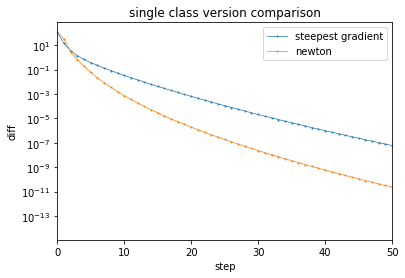
\includegraphics[width=10cm]{p1-1.png}
\end{figure}

\newpage
\subsection*{4 Multiclass version}
マルチクラスのデータセットに対しても、同様に最急降下法とニュートン法を実装した。両者を比較したグラフは上図のよう(multiclass version comparisoin)。

\begin{figure}
    \centering
    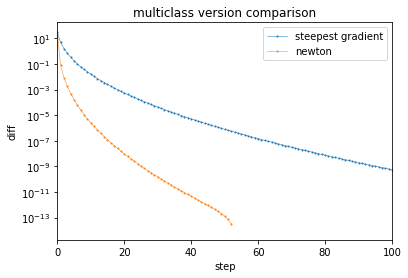
\includegraphics[width=10cm]{p1-4.png}
\end{figure}


\newpage
\section{PROBLEM 2}
本課題で作成したコードはgithub(\url{https://github.com/naoyaaan/AdvancedMachineLearning/tree/main/Shimosaka})に公開しています。
\begin{equation}
    \hat{w} = \argmin_{w} \left((w-\mu)^{T}A(w-\mu)+\lambda \|w\|_1\right)
\end{equation}
近接勾配法を用いて$\hat{w}$を求める。$J(w) = \left((w-\mu)^{T}A(w-\mu)+\lambda \|w\|_1\right)$とおくと、その勾配は以下のよう。

\begin{equation}
    \nabla J(w) = 2A(w-\mu)
\end{equation}

また、wの更新は以下の式のように行う。

\begin{eqnarray}
    w^{(t+1)} &=& prox_{\eta_t} \left(w^{(t)} - \eta\nabla J(w)\right)\\
    &=& prox_{\eta_t} \left(w^{(t)} - \frac{1}{L}2A(w-\mu)\right)
\end{eqnarray}

ここで、この問題ではL1 regularizationを考えているので、以下のようにproximal operationは表せる。

\begin{equation}
    prox_{q|\cdot|}(\mu) = ST_q(\mu)
\end{equation}

\begin{equation}
    ST_q(\mu) = \begin{cases}
        \mu-q & if~\mu > q \\
        0 & if~|\mu| \leq q \\
        \mu+q & if~\mu < -q
    \end{cases}
\end{equation}

上記を実装し、以下のグラフが得られた。
\begin{figure}[htbp]
    \centering
    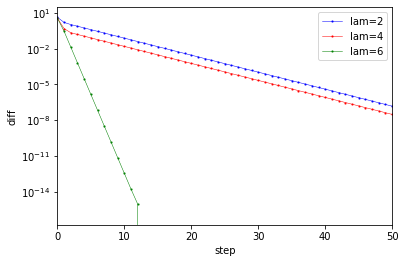
\includegraphics[width=100mm]{p2-4.png}
    \caption{result}
\end{figure}

\begin{figure}[htbp]
    \begin{minipage}{0.5\hsize}
     \begin{center}
      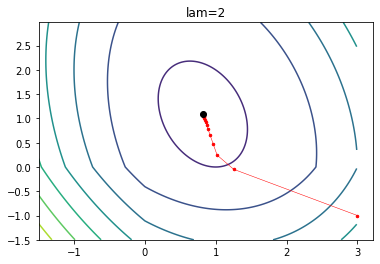
\includegraphics[width=70mm]{p2-1.png}
     \end{center}
    \end{minipage}
    \begin{minipage}{0.5\hsize}
     \begin{center}
      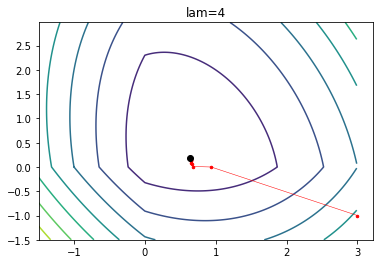
\includegraphics[width=70mm]{p2-2.png}
     \end{center}
    \end{minipage}
    \begin{minipage}{0.5\hsize}
     \begin{center}
      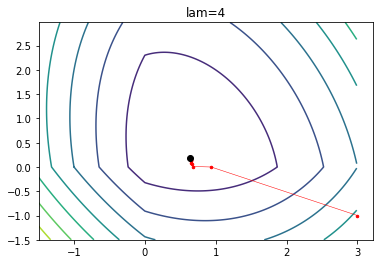
\includegraphics[width=70mm]{p2-2.png}
     \end{center}
    \end{minipage}
\end{figure}


\newpage
\section{PROBLEM 3}

\begin{equation}
    \hat{w} = \argmin_{w\in \mathbb{R}^d} \Biggl(\sum_{i=1}^{n}\max(0,1-y_iw^Tx_i) + \lambda \|w\|^2_2 \Biggr) \label{problem3}
\end{equation}

\subsection*{1, 2}
式(\ref{problem3})にスラック変数を導入して変形していくと、式(\ref{problem3})の問題は以下のような問題に変形できる。

\begin{equation}
    \begin{aligned}
        & \text{minimize}
            & \lambda w^Tw + 1^T\xi\\
        &\text{subject to}
            & \xi \geq 1-y_iw^Tx_i \text(,i = 1,...,n)\\
            & & \xi \geq 0\\
    \end{aligned}
\end{equation}

$\alpha \in \mathbb{R}^n$,$\beta \in \mathbb{R}^d$としてラグランジュ方程式を定義する。ここでKKT条件も考えると、以下のようになる。

\begin{equation}
    L(w,\xi,\alpha,\beta) = \lambda w^Tw + 1^T\xi + \sum_{i}\alpha (1-y_iw^Tx_i-\xi_i)-\beta^T\xi
\end{equation}

ラグランジュの導関数:
\begin{equation}
    \begin{aligned}
        &\frac{\partial L}{\partial w} = 2\lambda w- \sum_i \alpha_i y_i x_i
        &\Rightarrow 
        &&\hat{w} = \frac{1}{2\lambda}\sum_i\hat{\alpha}_i y_i x_i
    \end{aligned}
\end{equation}

\begin{equation}
    \begin{aligned}
        &\frac{\partial L}{\partial \xi} = 1-\alpha-\beta
        &\Rightarrow
        &&\hat{\alpha_i} + \hat{\beta_i} = 1 
        &&\text{i=1,...,n}
    \end{aligned}
\end{equation}

ラグランジュ変数の不等式 : $\hat{\alpha_i}\geq0$,$\hat{\beta_i}\geq0$

スラックの相補条件:
\begin{center}
    $\hat{\alpha}(1-\hat{\xi_i}-y_i\hat{w}^Tx_i) = 0$, i=1,...,n

    $\hat{\beta}\i \hat{\xi}\i = 0$, i=1,...,n
\end{center}

ここでラグランジュの双対問題を考えると
\begin{equation}
    \begin{aligned}
        & \text{maximize}_{\alpha}
            & -\frac{1}{4\lambda}\alpha^TK\alpha+1^T\alpha\\
        &\text{subject to}
            & 0\leq\alpha\leq 1
    \end{aligned}
\end{equation}

\begin{equation*}
    \{K\}_{i,j} = \sum_i y_i y_j x_i^T x_j
\end{equation*}

\begin{equation*}
    \hat{w} = \frac{1}{2\lambda}\sum_i \hat{\alpha}_i y_i x_i
\end{equation*}

\begin{equation*}
    \hat{\alpha_i} + \hat{\beta_i} = C
\end{equation*}

以上より、1,2の問題を示せた。

\subsection*{3}
本課題で作成したコードはgithub(https://github.com/naoyaaan/AdvancedMachineLearning)に公開しています。
\newpage
実装による計算結果として上図のようなグラフが得られた。
最初のグラフは、$w=\hat{w}$となるときのラグランジュ関数の値との差分の遷移を表したものである。
2つ目のグラフは、$w=\hat{w}$となるときのhinge loss関数の値との差分の遷移を表した物である。

\begin{figure}
    \centering
    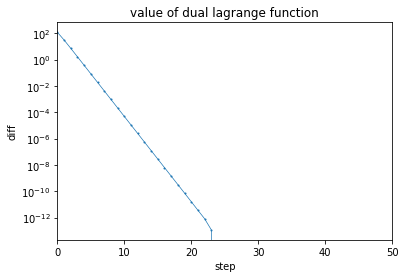
\includegraphics[width=10cm]{p3-3-1.png}
\end{figure}

\begin{figure}
    \centering
    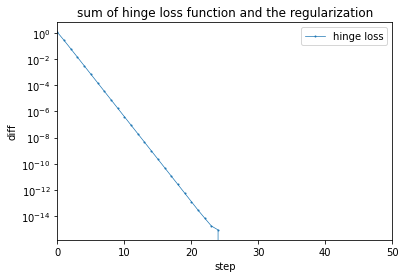
\includegraphics[width=10cm]{p3-3-2.png}
\end{figure}

\newpage
\section{PROBLEM 4}
\subsection*{1}
\begin{equation}
    \hat{w} = \argmin_{w\in \mathbb{R}^d} \Biggl(\sum_{i=1}^{n}\max(0,1-y_iw^Tx_i) + \lambda \|w\|_1 \Biggr) \label{problem4}
\end{equation}

式(\ref{problem4})にスラック変数($\xi_i \geq 1-y_iw^Tx_i \geq 0$,$e_i \geq |w_i| \geq 0$)を導入して変形していくと、式(\ref{problem4})の問題は以下のような問題に変形できる。

\begin{equation}
    \begin{aligned}
        & \text{minimize}
            &  1^T\xi + \lambda 1^Te\\
        &\text{subject to}
            & \xi \geq 1-y_iw^Tx_i \text(,i = 1,...,n)\\
            && \xi \geq 0\\
            && e_i \geq |w_i| 
    \end{aligned}
\end{equation}

\begin{equation*}
    L(w,\xi,\alpha,\beta,\gamma) = 1^T\xi + \lambda 1^Te + \sum_i \alpha_i(1-y_iw^Tx_i-\xi_i) - \beta^T\xi + \gamma(w-e) - \delta e
\end{equation*}

\begin{equation*}
    \frac{\partial L}{\partial e} = \lambda - \gamma - 1
\end{equation*}

\begin{equation*}
    \frac{\partial L}{\partial \xi} = 1-\alpha-\beta
\end{equation*}

\begin{equation*}
    \frac{\partial L}{\partial w} = \gamma - \sum_i \alpha_i y_i x_i
\end{equation*}

\begin{equation*}
    z :=
    \begin{pmatrix}
        \xi & e
    \end{pmatrix}
\end{equation*}

\begin{equation*}
    c :=
    \begin{pmatrix}
        1 & \lambda
    \end{pmatrix}
\end{equation*}

\begin{equation*}
    a :=
    \begin{pmatrix}
        1 & 0
    \end{pmatrix}
\end{equation*}

\begin{equation*}
    A :=
    \begin{pmatrix}
        Y & 1
    \end{pmatrix}
\end{equation*}

\begin{equation*}
    B := 1
\end{equation*}

\newpage
\section*{PROBLEM 8}
\subsection*{1}
まず、$\hat{w_{LS}}$について考える。

\begin{eqnarray}
    \hat{w_{LS}} &=& \argmin_{w} \frac{1}{2}||y-Xw||^2_2\\
    &=& \argmin_{w} \frac{1}{2}(y^Ty-2w^TX^Ty + w^TX^TXw)
\end{eqnarray}

ここで勾配を考える。

\begin{equation}
    \begin{aligned}
        & \frac{\partial L(w)}{\partial w}|_{w=\hat{w_{LS}}} = 0
        &\Rightarrow
        &&\frac{\partial L}{\partial w}|_{w=\hat{w_{LS}}} = -X^Ty + X^TX\hat{w} = 0\\
        &&\hat{w} = (X^TX)^{-1}X^Ty
    \end{aligned}
\end{equation}

以上より、$\hat{w_{LS}} = (X^TX)^{-1}X^Ty$となる。\\

次に、$\hat{w}_{ridge}$について考える。
\begin{eqnarray}
    \hat{w}_{ridge} &=& \argmin_{w} \frac{1}{2}||y-Xw||^2_2 + \lambda ||w||^2_2\\
    &=& \argmin_{w} \frac{1}{2}(y^Ty-2w^TX^Ty + w^TX^TXw) + \lambda ww^T
\end{eqnarray}

ここで勾配を考える。

\begin{equation}
    \begin{aligned}
        & \frac{\partial L(w)}{\partial w}|_{w=\hat{w}_{ridge}} = 0
        &\Rightarrow
        &&\frac{\partial L}{\partial w}|_{w=\hat{w}_{ridge}} = -X^Ty + (X^TX + \lambda I) \hat{w}= 0\\
    \end{aligned}
\end{equation}

以上より、$\hat{w}_{ridge} = (X^TX + \lambda I)^{-1}X^Ty$となる。

\subsection*{2}
$X^TX$は対象行列であるので直行行列$P(P^T = P^{-1})$で、
\begin{equation}
    \begin{aligned}
        X^TX = P\Gamma P^T 
        &(\Gamma = diag(\gamma_0,...,\gamma_D))
    \end{aligned}
\end{equation}
と対角化が可能である。よって以下のようになる。

\begin{eqnarray*}
    (X^TX + \lambda I)^{-1} &=& (P\Gamma P^T + \lambda I)^{-1}\\
    &=& \left( P(\Gamma + \lambda I)P^T \right))^{-1}\\
    &=& P(\Gamma + \lambda I )^{-1}P^T\\
    &=& Pdiag(\frac{1}{\gamma_0 + \lambda},\frac{1}{\gamma_1 + \lambda},...,\frac{1}{\gamma_D + \lambda})P^T
\end{eqnarray*}

最小の固有値がゼロのとき$\lambda > 0$であるので、収束する。よって$X^TX + \lambda I$は正則である。

% \subsection*{3}

\section*{講義資料の修正箇所について}
\subsection*{1つ目}
本課題のmidterm-assignment.pdfの資料のProblem 3 の第2問において、
\begin{equation*}
    \hat{w} = \frac{1}{2\lambda} \sum_{i=1}^n \alpha_i y_i x_i
\end{equation*}
と$\alpha_i$となっているが、ここでは
\begin{equation*}
    \hat{w} = \frac{1}{2\lambda} \sum_{i=1}^n \hat{\alpha}_i y_i x_i
\end{equation*}
のように$\hat{\alpha}_i$とするべきである。

\subsection*{2つ目}
第1回の資料、m1-03.pdfに修正箇所がある。p23において、「The optimal values $\hat{a},\hat{b},\hat{\sigma}$ are...」とあるが、ここでは、$\hat{\sigma}$ではなく、$\hat{\sigma}^2$とするべきである。

\end{document}